\subsection{Review of Base Systems and Mayan Numerals}


\content{
        \begin{example}
        Write the number $3042_5$ in base 10.        
        \end{example}
}{% presentation
\vspace{2in}
}{% nopresentation
\vspace{2in}
}{% comments
}

\content{
        \begin{example}
        Write the number $81173_9$ in base 10.        
        \end{example}
}{% presentation
\vspace{2in}
}{% nopresentation
\vspace{2in}
}{% comments
}

\content{
        \begin{example}
        Write $1024$ in base $6$.
        \end{example}
}{% presentation
\vspace{2in}
}{% nopresentation
\vspace{2in}
}{% comments
}

\content{
        \begin{example}
        Write $932$ in base 9.        
        \end{example}
}{% presentation
\vspace{2in}
}{% nopresentation
\vspace{2in}
}{% comments
}

\content{
        \begin{example}
        Write $721_8$ in base 10.        
        \end{example}
}{% presentation
\vspace{2in}
}{% nopresentation
\vspace{2in}
}{% comments
}

\content{
        \begin{example}
        Write $321_4$ in base 5. (Hint: first convert to base 10)
        \end{example}
}{% presentation
\vspace{2in}
}{% nopresentation
\vspace{2in}
}{% comments
}

\content{
        \begin{minipage}[t]{0.65\textwidth}
        \vspace{0pt}
        Recall the Mayan positional system.
        \begin{example}
        Write $35$ and $89$ in the Mayan numeral system, then compute their sum
        using that representation.
        \end{example}
        \end{minipage}\hfill
        \begin{minipage}[t]{0.3\textwidth}
        \vspace{0pt}
        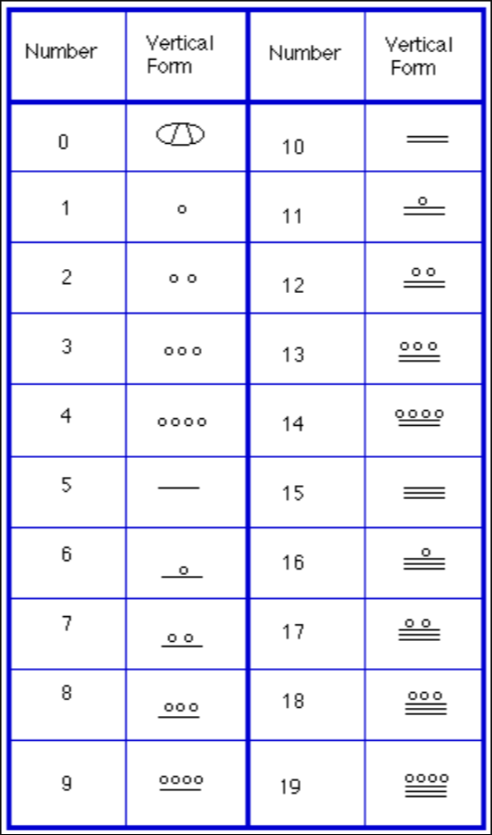
\includegraphics[scale=0.25]{mayan-symbols.png}
        \end{minipage}
}{% presentation
}{% nopresentation
}{% comments
}
